% IEEE conference version for GTSD 2026 proceedings
\documentclass[conference]{IEEEtran}
\usepackage{cite}
\usepackage{amsmath,amssymb,amsfonts}
\usepackage{graphicx}
\graphicspath{{figures/}}
\usepackage{textcomp}
\usepackage{booktabs}
\usepackage{algorithm}
\usepackage{algpseudocode}
\usepackage{url}
\def\BibTeX{{\rm B\kern-.05em{\sc i\kern-.025em b}\kern-.08em
    T\kern-.1667em\lower.7ex\hbox{E}\kern-.125emX}}

\begin{document}
\bstctlcite{IEEEexample:BSTcontrol}

% Initialize section counter to 2 so this section compiles cleanly as Section III (Part 2: III-D Overlap-Tiling)
\setcounter{section}{2}
\section{Proposed Hardware-Software Co-Design Framework (Cont. --- Overlap-Tiling)}

% Initialize counters to maintain seamless continuity with Part 1 (III-A, III-B, III-C)
\setcounter{subsection}{3} % Next subsection will be III-D
\setcounter{equation}{10}  % Next equation will be (11)
\setcounter{figure}{4}    % Next figure will be Fig. 5

% =========================================================================
% III-D. HARDWARE-AWARE OVERLAP-TILING & BOUNDARY ARTIFACT ELIMINATION
% =========================================================================
\subsection{Hardware-Aware Overlap-Tiling and Boundary Artifact Elimination}
\label{sec:tiling}

High-resolution clinical radiographs routinely span dimensions from $1024 \times 1024$ to over $2048 \times 2048$ pixels. Buffering an entire high-resolution frame on-chip alongside intermediate feature tensors requires tens of megabytes of fast memory, far exceeding the total Block RAM budget of edge-class SoCs (the target Zynq-7020 fabric provides only 140 BRAM36K blocks, equivalent to $\approx 630$~KB or 4.92~Mb) \cite{sze2017efficient, mittal2020survey}. Consequently, inference must be executed using a tile-by-tile streaming strategy. 

However, partitioning an image into isolated non-overlapping blocks introduces severe boundary distortions. Valid 2D convolutions shrink spatial boundaries unless zero-padding is applied; yet, applying zero-padding at tile perimeters introduces artificial dark boundary values that propagate across cascading layers, causing prominent step discontinuities known as \textit{blocking artifacts} along reconstruction seams. To resolve this dilemma, we develop a mathematically rigorous, hardware-aware \textbf{Overlap-Tiling} and stitching pipeline \cite{peemen2013memory}.

\begin{figure}[t]
\centering
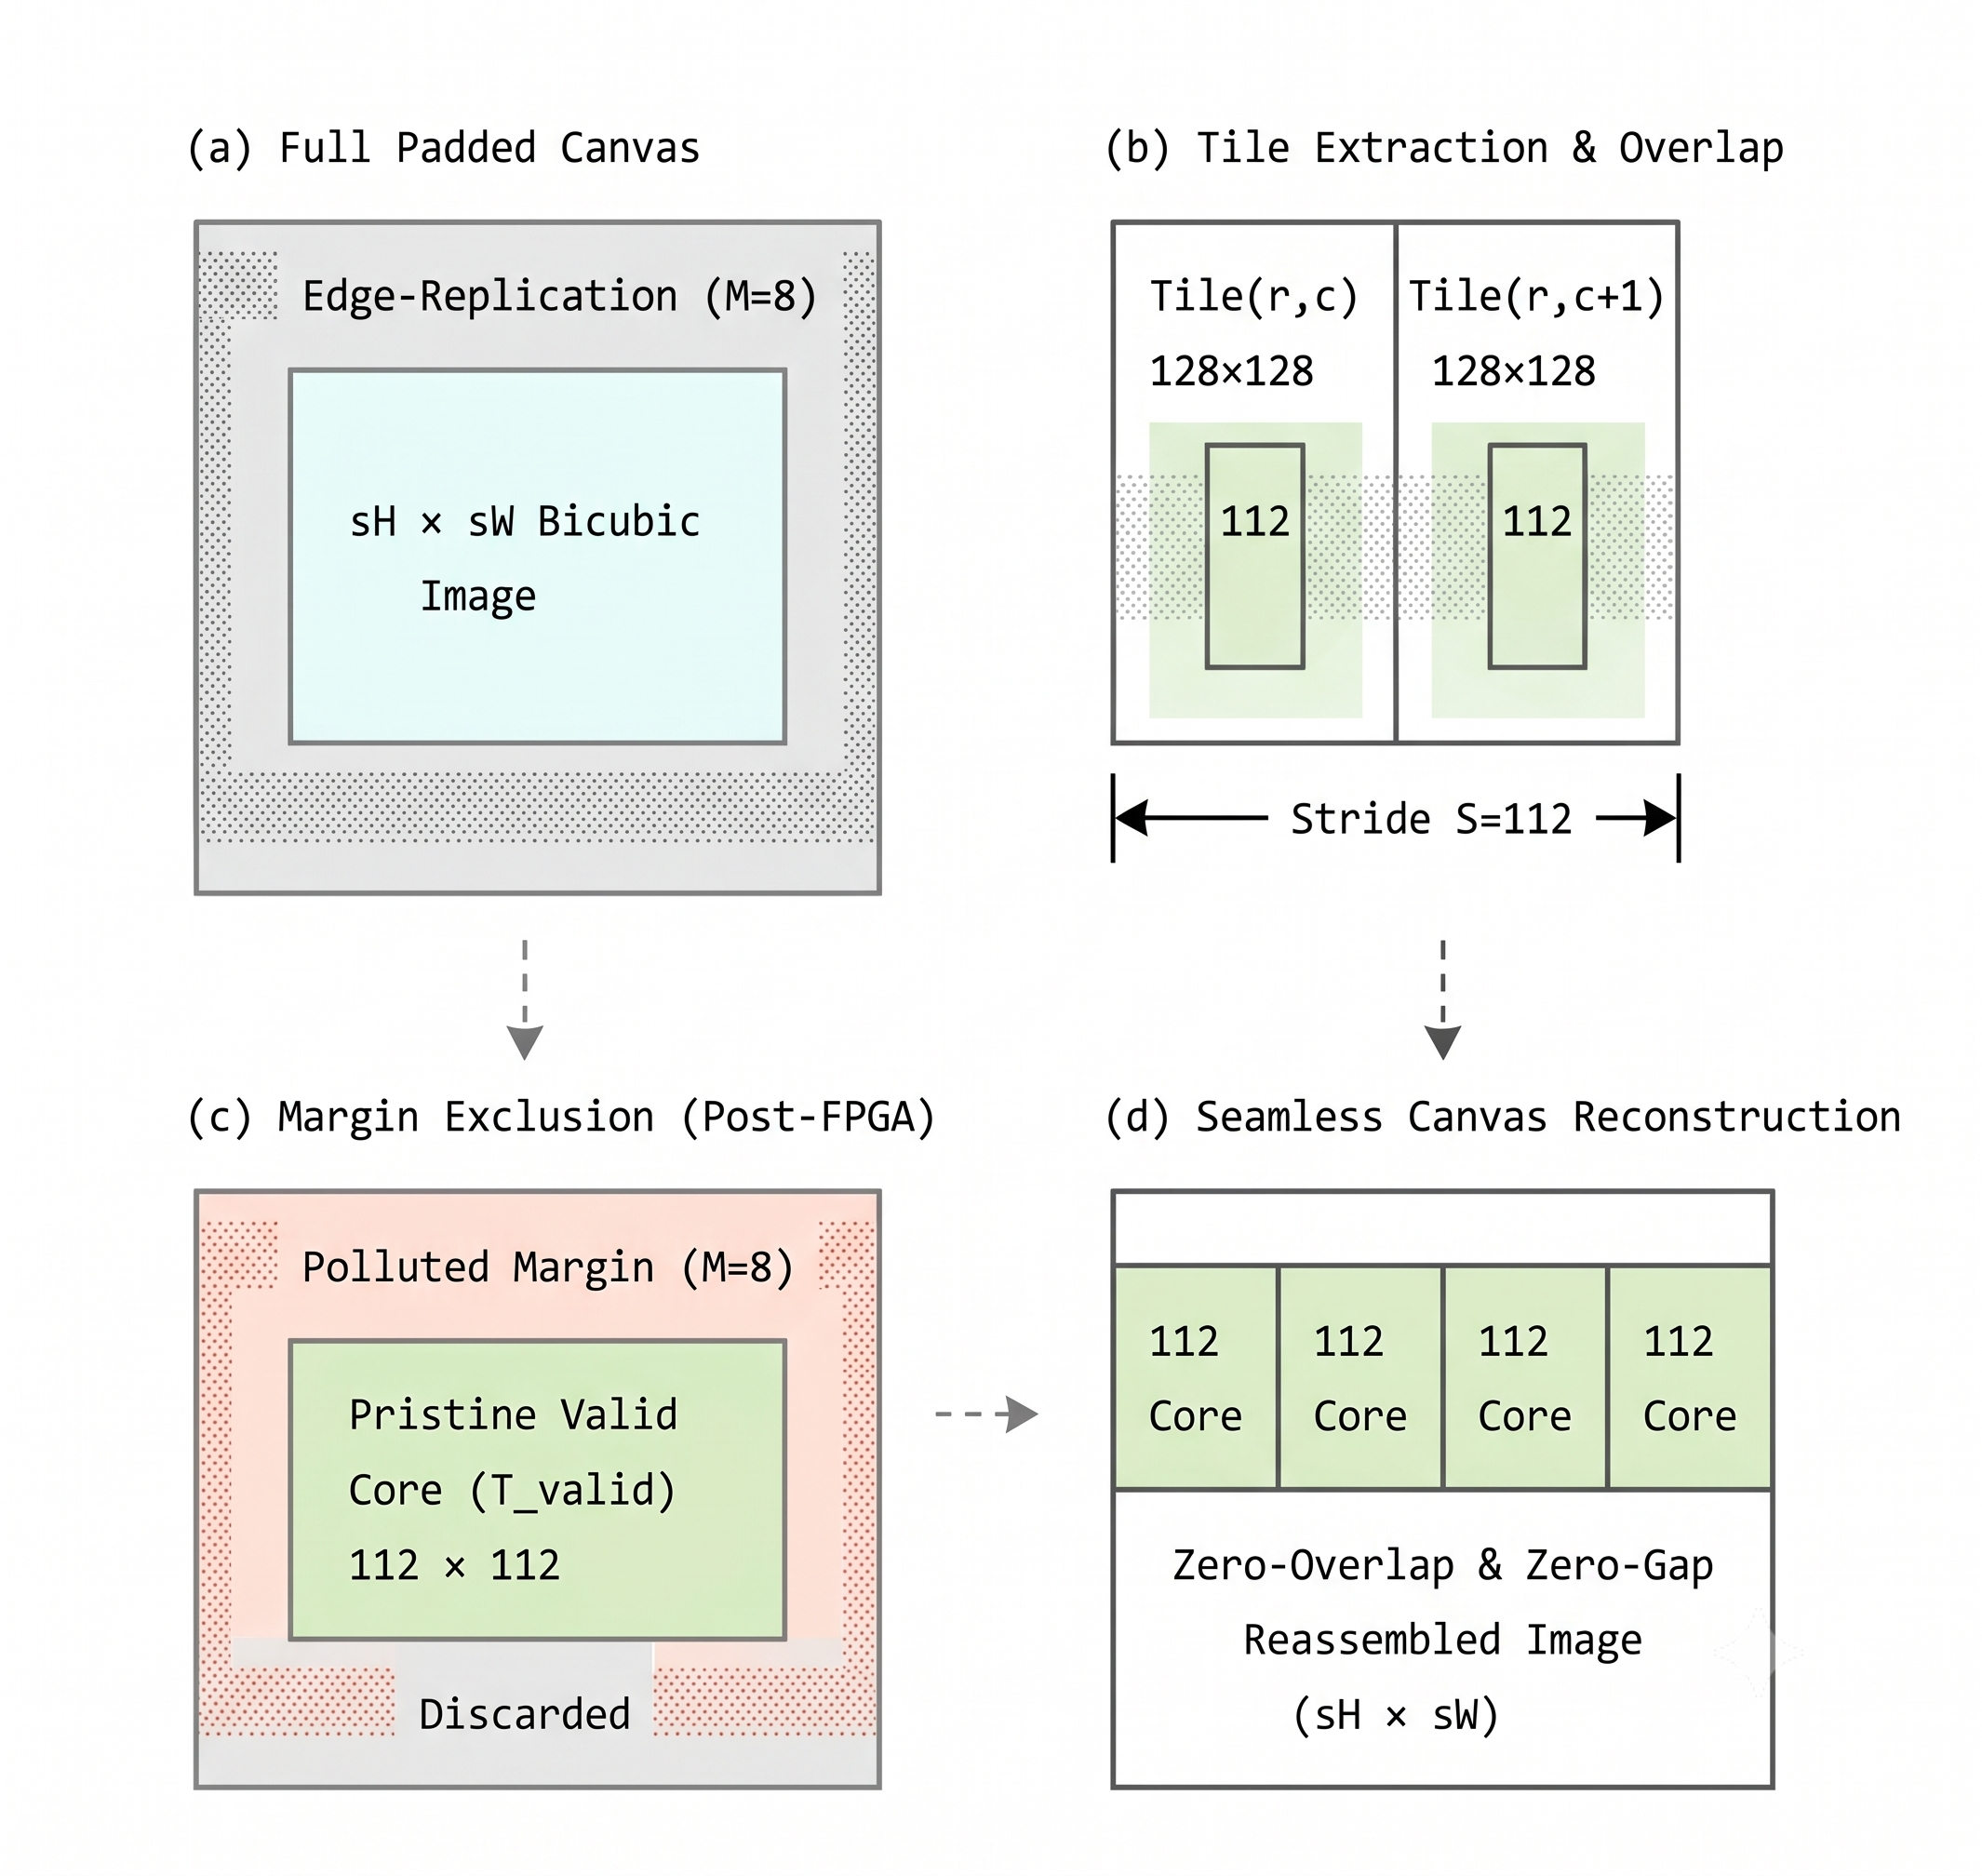
\includegraphics[width=\columnwidth]{overlap_tiling_mechanism.png}
\caption{Hardware-aware overlap-tiling strategy: (a) Input image extension via edge-replication padding, (b) Partitioning into $P \times P = 128 \times 128$ overlapping tiles with stride $S = 112$ and margin $M = 8$, (c) Accelerator processing and extraction of the pristine $112 \times 112$ valid core ($T_{valid}$), and (d) Seamless, artifact-free canvas reassembly.}
\label{fig:overlap_tiling}
\end{figure}

\subsubsection{Theoretical Receptive Field and Margin Derivation}
The spatial distortion halo produced by unpadded convolutions is strictly bounded by the network's theoretical receptive field. For a cascade of $L$ convolutional layers with spatial kernel dimensions $K_l \times K_l$ ($l \in \{1, 2, \dots, L\}$) and unit strides, the cumulative receptive field $R$ is formulated as:
\begin{equation}
R = 1 + \sum_{l=1}^L (K_l - 1)
\label{eq:receptive_field}
\end{equation}
For our compact 3-layer SRCNN with kernel sizes $K_1 = 9$, $K_2 = 1$, and $K_3 = 5$, the cumulative receptive field evaluates to:
\begin{equation}
R = 1 + (9 - 1) + (1 - 1) + (5 - 1) = 13\text{ pixels}
\label{eq:receptive_field_calc}
\end{equation}
Because spatial convolution symmetrically aggregates neighborhood information around each target coordinate, any output pixel situated within a boundary distance less than:
\begin{equation}
M_{min} = \frac{R - 1}{2} = \frac{13 - 1}{2} = 6\text{ pixels}
\label{eq:margin}
\end{equation}
receives incomplete receptive field support. Pixels within this $6$-pixel boundary margin suffer from boundary distortion and must be discarded.

To facilitate power-of-two memory alignment and align with 64-bit AXI DMA burst transfers, we conservatively configure a boundary margin of $M = 8\text{ pixels}$ ($M > M_{min}$). Fixing the physical accelerator tile buffer to $P \times P = 128 \times 128$ pixels yields an effective, distortion-free \textbf{valid core stride} $S$:
\begin{equation}
S = P - 2M = 128 - 2(8) = 112\text{ pixels}
\label{eq:stride}
\end{equation}
By stepping across the image at intervals of exactly $S = 112$ pixels, the valid cores seamlessly tile the target image space without gaps or overlapping redundancies, as illustrated in Fig.~\ref{fig:overlap_tiling}.

\subsubsection{Global Canvas Partitioning and True Boundary Padding}
For an input radiograph $I_{LR} \in \mathbb{R}^{H \times W}$ scaled by factor $s = 2$ to bicubic target size $sH \times sW$, the required number of tile rows $N_R$ and columns $N_C$ is determined by:
\begin{equation}
N_R = \left\lceil \frac{sH}{S} \right\rceil, \quad N_C = \left\lceil \frac{sW}{S} \right\rceil
\label{eq:tile_grid}
\end{equation}
To ensure that boundary tiles at the image perimeter have sufficient spatial context, the global image is extended into an expanded canvas buffer of dimension $H_{pad} \times W_{pad}$:
\begin{equation}
H_{pad} = N_R \cdot S + 2M, \quad W_{pad} = N_C \cdot S + 2M
\label{eq:canvas_pad}
\end{equation}

Crucially, while interior tile borders overlap and have their margins discarded, the outermost perimeter of the full radiograph has no adjacent neighboring patches. To completely eliminate step discontinuities at the outer image borders, we implement \textbf{edge-replication padding}:
\begin{equation}
I_{pad}(y, x) = I_{bic}\left(\text{clamp}(y - M,\, 0,\, sH - 1),\, \text{clamp}(x - M,\, 0,\, sW - 1)\right)
\label{eq:edge_pad}
\end{equation}
where $0 \le y < H_{pad}$ and $0 \le x < W_{pad}$. Edge replication extends the outermost anatomical pixel intensities outward, preventing artificial contrast gradients from masquerading as peripheral pathological lesions.

\subsubsection{Streaming Orchestration Algorithm}
The end-to-end tiling, hardware streaming, and reconstruction flow is formalized in Algorithm~\ref{alg:tiling_dma}. The host software slices the padded canvas into $128 \times 128$ tiles, formats them into signed S7.0 representation, and dispatches them across the AXI DMA interface. Upon receiving the accelerated $128 \times 128$ output from the PL, the host crops the center $112 \times 112$ valid core $T_{valid}$ and commits it to the output canvas $I_{canvas}$. Once all $N_R \times N_C$ tiles are processed, the unpadded $sH \times sW$ region is extracted, yielding a continuous, mathematically exact super-resolved radiograph without blocking seams.

\begin{algorithm}[t]
\caption{Hardware-Aware Overlap-Tiling and DMA Streaming}
\label{alg:tiling_dma}
\begin{algorithmic}[1]
\Require Low-resolution radiograph $I_{LR} \in \mathbb{R}^{H \times W}$, scale factor $s = 2$, tile size $P = 128$, stride $S = 112$, margin $M = 8$.
\Ensure Super-resolved reconstructed radiograph $I_{SR} \in \mathbb{R}^{sH \times sW}$.
\State $I_{bic} \leftarrow \text{BicubicInterpolation}(I_{LR},\, s)$ \Comment{Scale to $sH \times sW$}
\State $N_R \leftarrow \lceil sH / S \rceil, \quad N_C \leftarrow \lceil sW / S \rceil$ \Comment{Grid dimensions}
\State $H_{pad} \leftarrow N_R \cdot S + 2M, \quad W_{pad} \leftarrow N_C \cdot S + 2M$
\State $I_{pad} \leftarrow \text{EdgeReplicationPad}(I_{bic},\, H_{pad},\, W_{pad},\, M)$
\State Initialize reconstruction canvas $I_{canvas} \in \mathbb{R}^{H_{pad} \times W_{pad}}$
\For{$r = 0$ \textbf{to} $N_R - 1$}
    \For{$c = 0$ \textbf{to} $N_C - 1$}
        \State $y \leftarrow r \cdot S, \quad x \leftarrow c \cdot S$
        \State $T_{in} \leftarrow I_{pad}[y : y + P,\, x : x + P]$ \Comment{Extract $128 \times 128$ tile}
        \State $T_q \leftarrow \text{clamp}(T_{in} - 128,\, -128,\, 127)$ \Comment{Cast to signed S7.0}
        \State $\text{AXI\_DMA\_Send}(T_q)$ \Comment{Stream input tile to PL}
        \State $T_{out} \leftarrow \text{AXI\_DMA\_Receive}()$ \Comment{Receive $128 \times 128$ from PL}
        \State $T_{valid} \leftarrow T_{out}[M : P - M,\, M : P - M]$ \Comment{Crop $112 \times 112$ core}
        \State $I_{canvas}[y + M : y + M + S,\, x + M : x + M + S] \leftarrow $ \Statex \hspace{4.2em} $T_{valid}$
    \EndFor
\EndFor
\State $I_{SR} \leftarrow I_{canvas}[M : M + sH,\, M : M + sW]$ \Comment{Crop valid frame}
\State \Return $I_{SR}$
\end{algorithmic}
\end{algorithm}

\bibliographystyle{IEEEtran}
\bibliography{bib/references}
\end{document}
